
% Chapter 1
\chapter{Introduction} % Main chapter title

\label{Introduction} % For referencing the chapter elsewhere, use \ref{Chapter1} 

\lhead{\emph{Introduction}} % This is for the header on each page - perhaps a shortened title

%----------------------------------------------------------------------------------------
\textbf{\emph{Rectilinear Polygons}} are a simple connected single-cyclic graph in $\mathbb{R}$$\times$$\mathbb{R}$, such that each of its edge is perpendicular or in-line with another one of its edge(s).

We encounter rectilinear polygons in various fields and applications such as network desgining, computer graphics, databases, VLSI Layout and image processing. The functions to be performed on rectilinear polygons are often more easily performed using either a rectangle partition or a rectanglular cover. In either case the rectilinear polygon is decomposed into a set of rectangles whose union is the original rectilinear polygon. If every two elements in the set of rectangles are disjoint, then it the set is called as a \emph{partition}.
\begin{figure}[h]
	\centering
    \scalebox{.5}{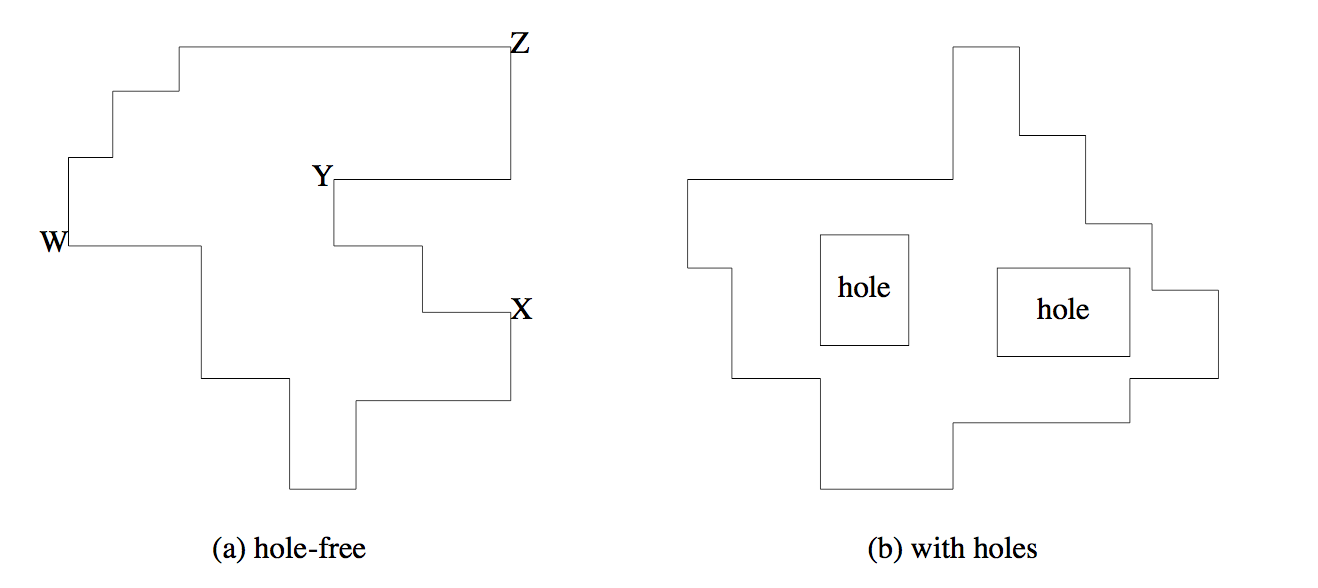
\includegraphics{Figures/fig1}}
    \caption{ Rectilinear Polygons [1]}
    \label{fig:Rect poly}
\end{figure}

A \textbf{\emph{minimal non-overlapping cover}} of a rectilinear polygon P is a rectangle partition of P that contains the fewest possible number of rectangles. The paper discusses a new complexity measure for the hole free rectilinear polygons. The paper defines the number of \emph{horizontal inversions, $k_{H}$} to be twice the minimum number of changes in horizontal motion while traveling around the polygon once. Similarly, the number of \emph{vertical inversions, $k_{V}$} to be twice the minimum number of changes in vertical motion while traveling around the polygon once.

The main complexity factor is \emph{k} which is given by
\begin{displaymath}
	 k = \min \{k_H, k_V\}
\end{displaymath}
This complexity measure covers a wide variety of polygons. The paper analysed 2869 polygons of which 85\% had \emph{k = 1} and 95\% had \emph{k $\leq$ 2}. Thus, for most practical reasons the \emph{O(kn)} algorithm is linear in time.
\\
\begin{figure}[h]
	\centering
	\scalebox{0.7}{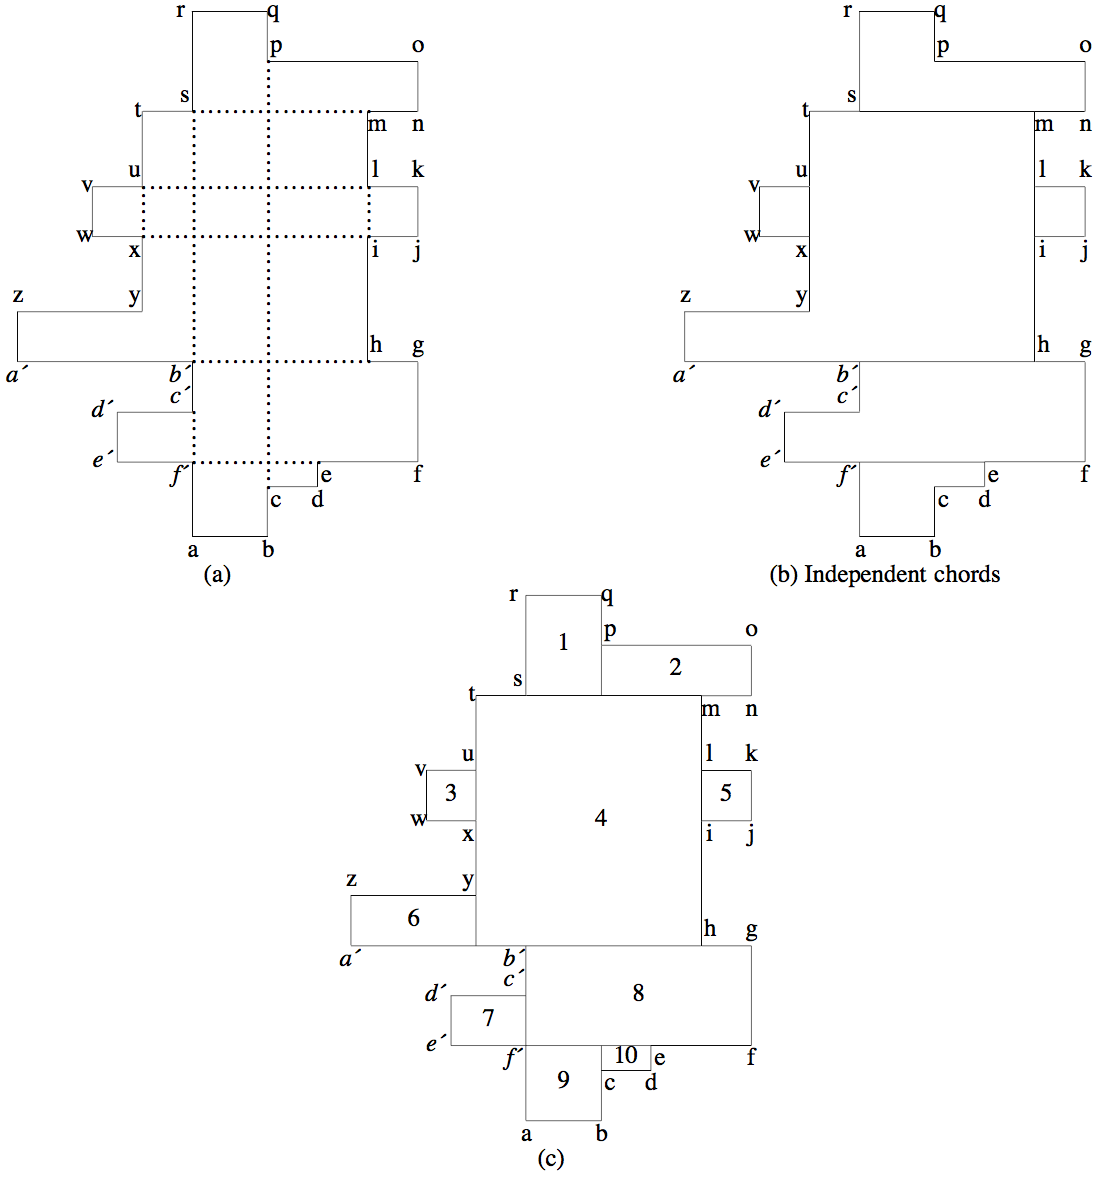
\includegraphics{Figures/fig2}}
	\caption{ Maximum Non-overlapping cover of a rectilinear polygon [1]}
	\label{fig:max cover}
\end{figure}
%----------------------------------------------------------------------------------------

\chapter{Definitions}
\label{Definitions}
\lhead{\emph{Definitions}}

\flushleft
\begin{enumerate}
	\item \textbf{Concave Vertices:} A vertex is said to be concave if the two edges intersecting at it makes an angle of $270^{\circ}$ with the interior of the polygon. For example, in Figure~\ref{fig:max cover}, the set of concave vertices  = \{c, h, i, l, m, p , s\}
	\item \textbf{Convex Vertices:} A vertex is said to be concave if the two edges intersecting at it makes an angle of $90^{\circ}$ with the interior of the polygon. For example, in Figure~\ref{fig:max cover}, the set of convex vertices = \{a, b, e, f\}
	\item \textbf{Chords: }A chord is a line joining any two co-horizontal concave vertices.
	\item \textbf{NEB(v): }Neighbourhood of a vertex v of a graph is defined as the set of all vertices, that have an edge incident from that vertex.
	\item \textbf{Convex Bipartite Graph: }A bipartite graph is said to be convex in V, if \forall{} v \in{}V, we can write it as a closed interval of the form [FIRST(v), LAST(v)]. In a convex bipartite graph labeling is crucial and needs to be defined for all problems together.
\begin{figure}[h]
	\centering
	\scalebox{0.45}{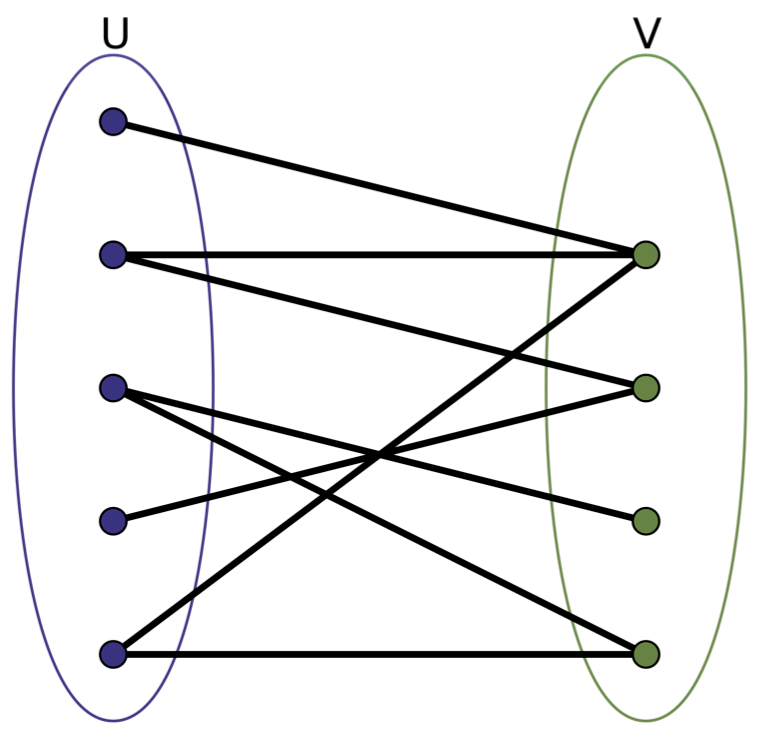
\includegraphics{Figures/fig3}}
	\caption{Convex Bipartite Graph on \emph{V} [4]}
	\label{fig:convex bipartite}
\end{figure}
  \item \textbf{Matchable vertex:} A vertex is matchable iff \exists y \in{} \emph{NEB(x)} such that,\emph{NEB(y)} \subseteq \emph{NEB(z)}, \forall z \in \emph{NEB(x)}.
  \item \textbf{Maximum Partition:} Partition of given rectillinear polygon into maximum number of non-overlapping rectangles.
  \item \textbf{Minimum Partition:} Partition of given rectillinear polygon into minimum number of non-overlapping rectangles, such that any two rectangles obtained , if merged will not form a rectangle.
\end{enumerate}

%----------------------------------------------------------------------------------------

\chapter{The Algorithm}
\label{The Algorithm}
\lhead{The Algorithm}
The algorithm is divided into multiple steps. The report reviews each step and the way of accepting input from the user, with a simple example.
\section{Method of Labelling the graph}
We take input as a rectilinear polygon from cursor keys, i.e., up($\uparrow$), left($\leftarrow$), and right ($\rightarrow$). As input is read, the pointer proceeds forward and draws a rectilinear polygon with its trail. The labelling of the vertices starts from $v_0$ to $v_{n-1}$, and $v_0 = v_n$, where n is the number of vertices in the polygon.

\begin{figure}[h]
	\centering
	\scalebox{0.5}{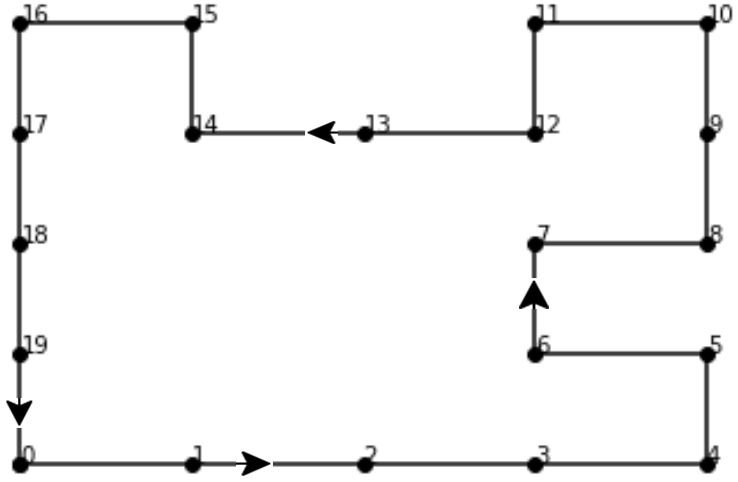
\includegraphics{Figures/fig6.png}}
	\caption{A Rectillinear polygon consisting of 20 vertices with direction of construction [5]}
	\label{fig:Rect poly example}
\end{figure}
\newpage
% --------------------------------------------------------
\section{INPUTS}
\textbf{G} = Rectilinear Graph \newline
\textbf{X} = Set of Abscissa of vertices \newline
\textbf{Y} = Set of Ordinates of vertices \newline
\textbf{Collinear\_Vertices} = Set of Collinear Vertices \newline
\textbf{Concave\_Vertices} = Set of Concave Vertices \newline
\textbf{Horizontal\_Chords} = Set of Horizontal Chords \newline
\textbf{Vertical\_Chords} = Set of Vertical Chords \newline

\underline{Important points to note}
\begin{enumerate}
\item Left and Right operations changes the direction the pointer faces.
\item Vertices that are induced after going forward consecutively. Although in the example, they are not explicitly shown,               but they do exist and at a distance of one unit from its previous vertex.
\item If the interior angle made by the two edges incident at this vertex is 270 degree.
\item Chords are lines joining two vertices which are not already part of the polygon.
\item As, the way of labelling is defined, there is unique labelling of each rectillinear polygon.
\end{enumerate}

\textbf{\emph{EXAMPLE:}}\\
In Figure~\ref{fig:Rect poly example}, the pointer is shown by an arrow. \newline
Total number of vertices = 20 \\
Collinear\_Vertices = [$v_{1}$, $v_{2}$, $v_{3}$, $v_{9}$, $v_{13}$, $v_{17}$, $v_{18}$, $v_{19}$] \\
Concave\_Vertices = [$v_{6}$, $v_{7}$, $v_{12}$, $v_{14}$] \\\*



\pagebreak
% --------------------------------------------------------

\section{Steps of Finding Maxiumum Partition}
\subsection{Step I}
\begin{lstlisting}
max_partition(G):
    for u in Concave_Vertices:
        for v in Concave_Vertices and v > u+1:
            if exists a chord joining v & u and ~exists another concave 
             vertex on chord joining v & u:
                if chord is horizontal: 
                    add (v, u) to Horizontal_Chords
                else if chord is vertical:
                    add (v, u) to Vertical_Chords
            else :
                loop_back
\end{lstlisting}
\textbf{Task Achieved:} All the edges that exist between \emph{any two concave vertices} are being added to their \emph{respectful categories}. \\
\textbf{\emph{EXAMPLE:}}\\
\begin{figure}[h]
  \centering
  \scalebox{0.5}{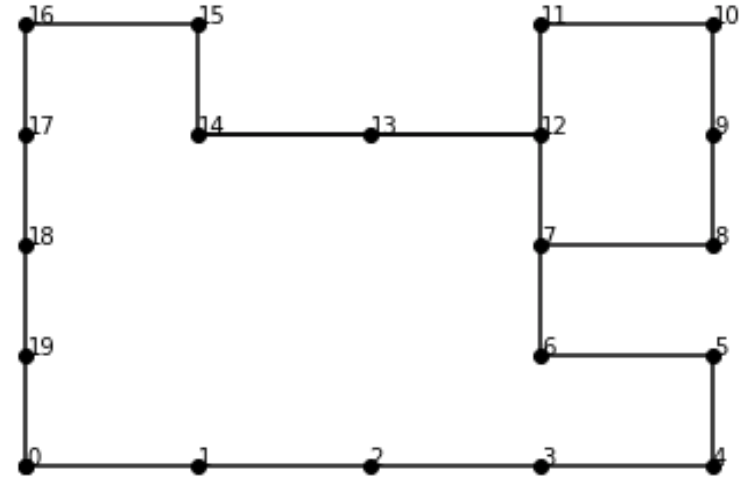
\includegraphics{Figures/fig5.png}}
\end{figure}

Horizontal\_Chords = \phi \\
Vertical\_chords = [($v_7$, $v_{12}$)] \\
\underline{Explanation:}
\textbf{u $>$ v :}Comparison between two vertices is done on the basis of their respective vertex indices. \
Here \textbf{v-u} should be greater than unity, because this assures the vertex v is not consecutive to u and has a higher index than u. Thus, iteration through each pair of vertex is done only once, making it more efficient. 

In the above code, we iterate through all (concave vertex, concave vertex') pairs, and check for existence of vertical and horizontal chords, that are not intersected by any other vertex.
We observe that, $v_7$ and $v_{12}$ are the only two concave vertices and between whom, there exists a vertical chord. Therefore, it is added to the set of \emph{Vertical\_Chords}. Also, there does not exist any horizontal chord between any two concave vertices and therefore, set of \emph{Horizontal\_Chords} is empty. \\

%----------------------------------------------------------
\subsection{Step II} % (fold)
\label{sub:step_2}
\begin{lstlisting}
 for u in Collinear_Vertices:
      for v in Concave_Vertices:
          if exists a chord joining v & u and ~exists another concave 
              or collinear vertex on chord joining v & u:
              if chord is horizontal:
                  add (v, u) to Horizontal_Chords
              else if chord is vertical:
                  add (v, u) to Vertical_Chords
          else :
              loop_back
\end{lstlisting}
\textbf{Task Achieved:} All the chords between \emph{collinear vertices and concave vertices} are being added to their \emph{respective categories}. 

\begin{figure}[h]
  \centering
  \scalebox{0.5}{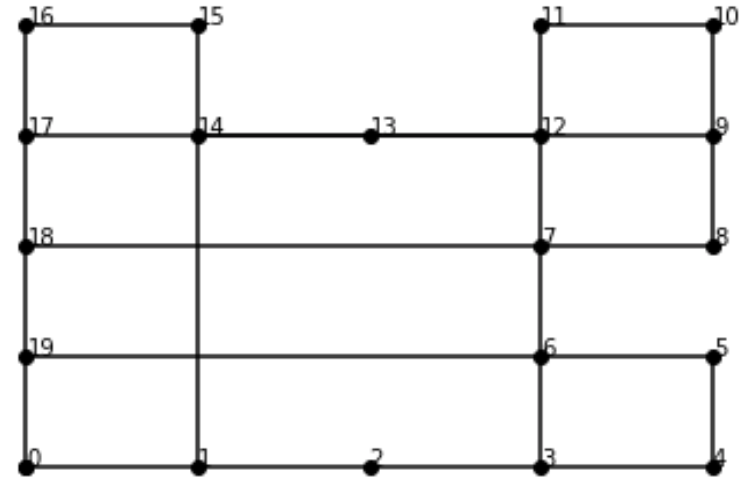
\includegraphics{Figures/fig4.png}}
\end{figure}

\emph{Horizontal\_Chords} =  [($v_{9}$, $v_{12}$), ($v_{17}$, $v_{14}$), ($v_{18}$, $v_{7}$), ($v_{19}$, $v_{6}$)] \\
\emph{Vertical\_Chords} =  [($v_{7}$, $v_{12}$), ($v_{1}$, $v_{4}$), ($v_{3}$, $v_{6}$)] 

\underline{Explanation}:
In the above code, we iterate through all (collinear vertex, concave vertex) pairs, and check for existence of vertical and horizontal chords between them, that are not intersected by any other vertex. \
If any chord is found, it is added to set of \emph{Vertical\_Chords or Horizontal\_Chords}, depending on its orientation. 

%----------------------------------------------------------
\subsection{Step III}

Thus, we have found all the chords, and only need to plot them now.

\begin{lstlisting}
    plot(X,Y)
    plot(Horizontal_Chords)
    plot(Vertical_Chords)
    display(plot)
\end{lstlisting}

\begin{figure}[h]
  \centering
  \scalebox{0.5}{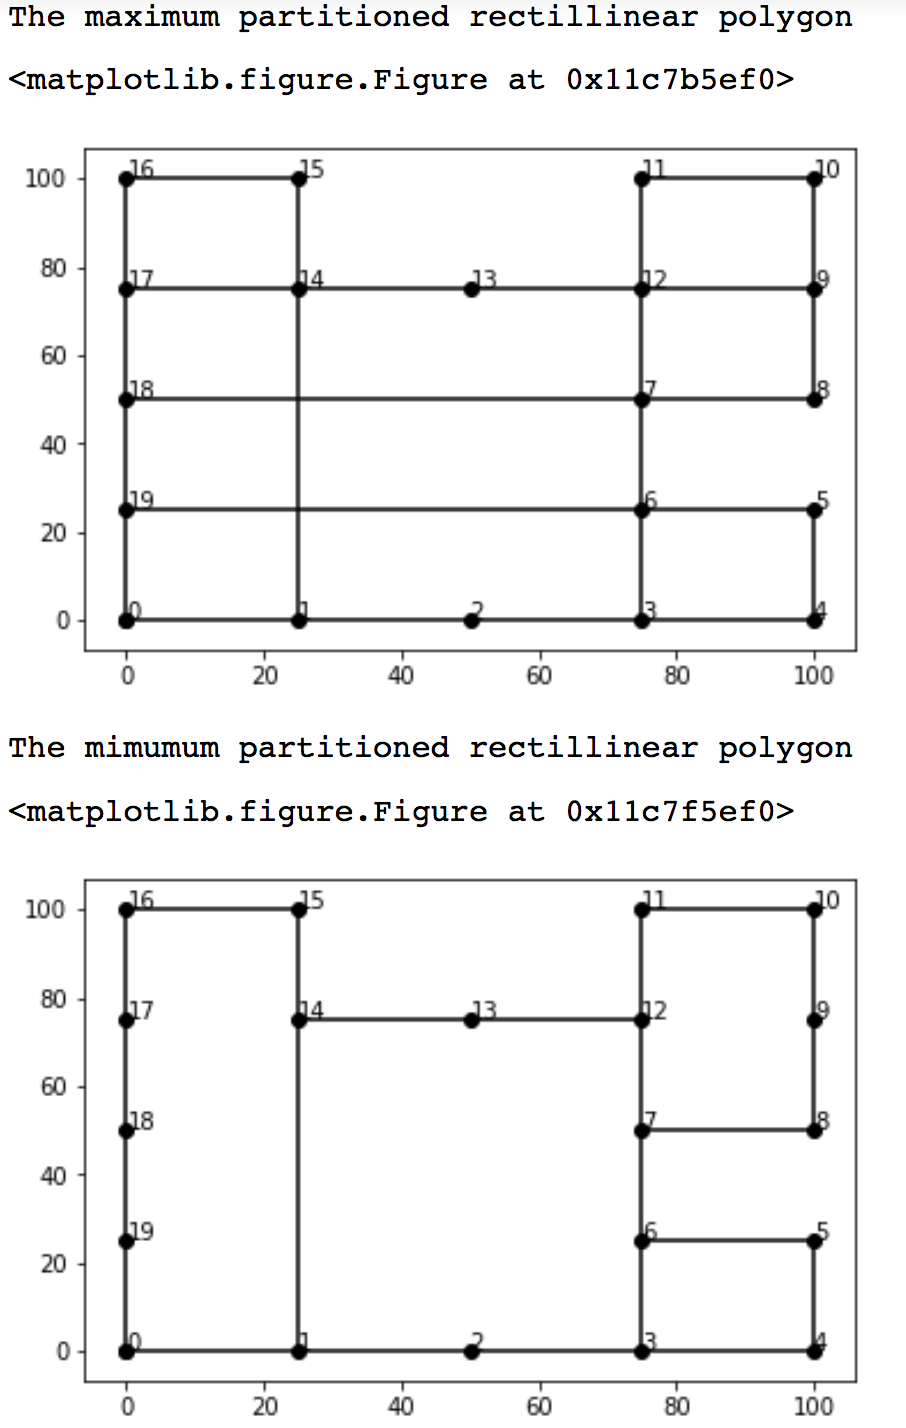
\includegraphics{Figures/fig7.png}}
\end{figure}
%----------------------------------------------------------

\subsection{Step IV}

Now we have found the maximum partition, but to find the minimum partition the following needs to be done
\begin{enumerate}
  \item Find a maximum independent set of chords (i.e., a maximum cardinality set of independent chords).
  \item Draw the chords in this maximum independent set. This partitions the polygon into smaller rectilinear polygons.
\end{enumerate}
%----------------------------------------------------------
\pagebreak
\subsection{Step V}
From each of the concave vertices from which a chord was not drawn in \emph{Step IV} draw a maximum length vertical line that is wholly within the smaller rectilinear polygon created in \emph{Step III} that contains this vertex.

%----------------------------------------------------------

\subsection{Step VI}

Thus, we have found all the chords, and only need to plot them now.
\begin{lstlisting}
    plot(X,Y)
    plot(Horizontal_Chords)
    plot(Vertical_Chords)
    plot(Nearest_Partial_Chords)
    display(plot)
\end{lstlisting}
%----------------------------------------------------------
\pagebreak

\section {Test Cases}

\textbf{INPUT 1}

\begin{figure}[h]
  \centering
  \scalebox{0.45}{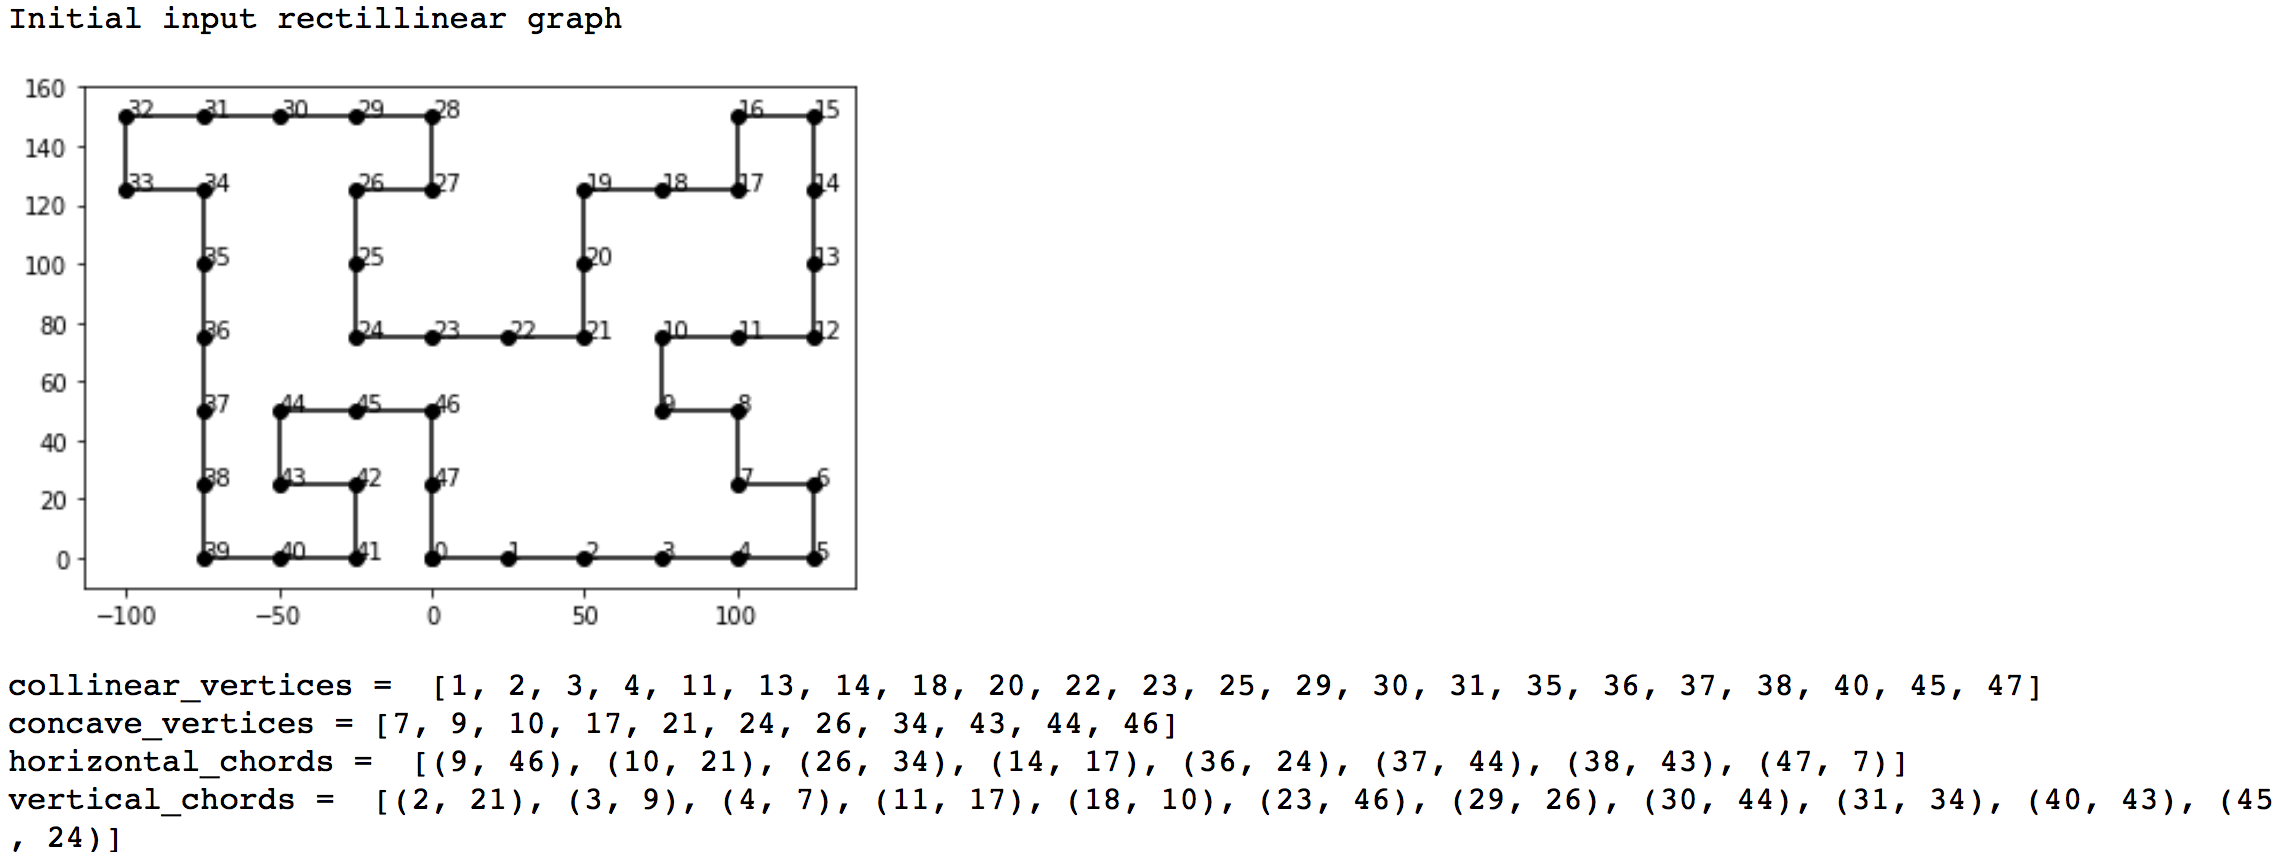
\includegraphics{Figures/t11.png}}
\end{figure}

\textbf{OUTPUT 1} 

\begin{figure}[h]
  \flushleft
  \scalebox{0.5}{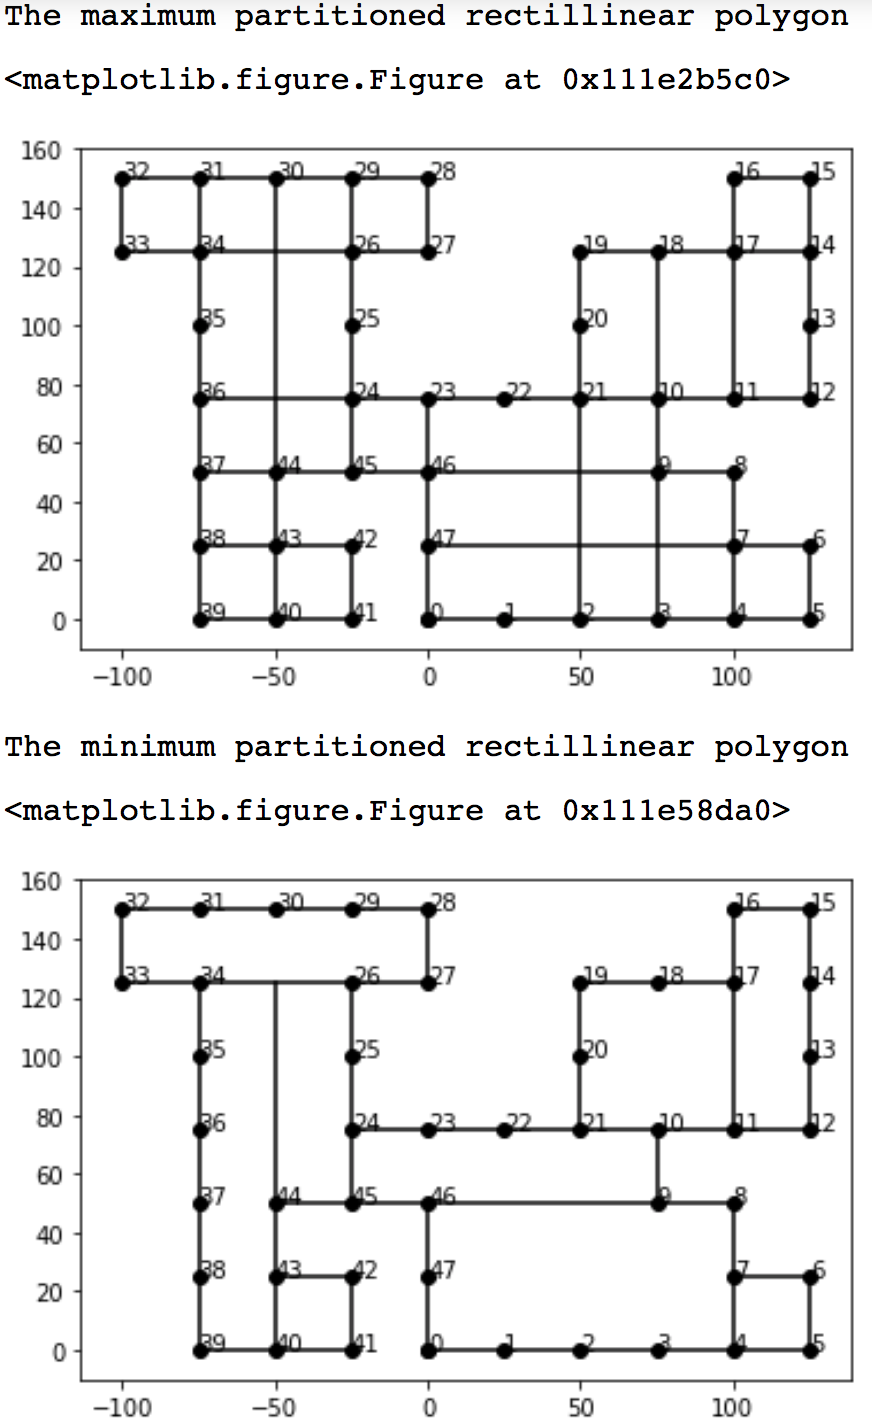
\includegraphics{Figures/t12.png}}
\end{figure}

\pagebreak
\textbf{INPUT 2}

\begin{figure}[h]
  \centering
  \scalebox{0.45}{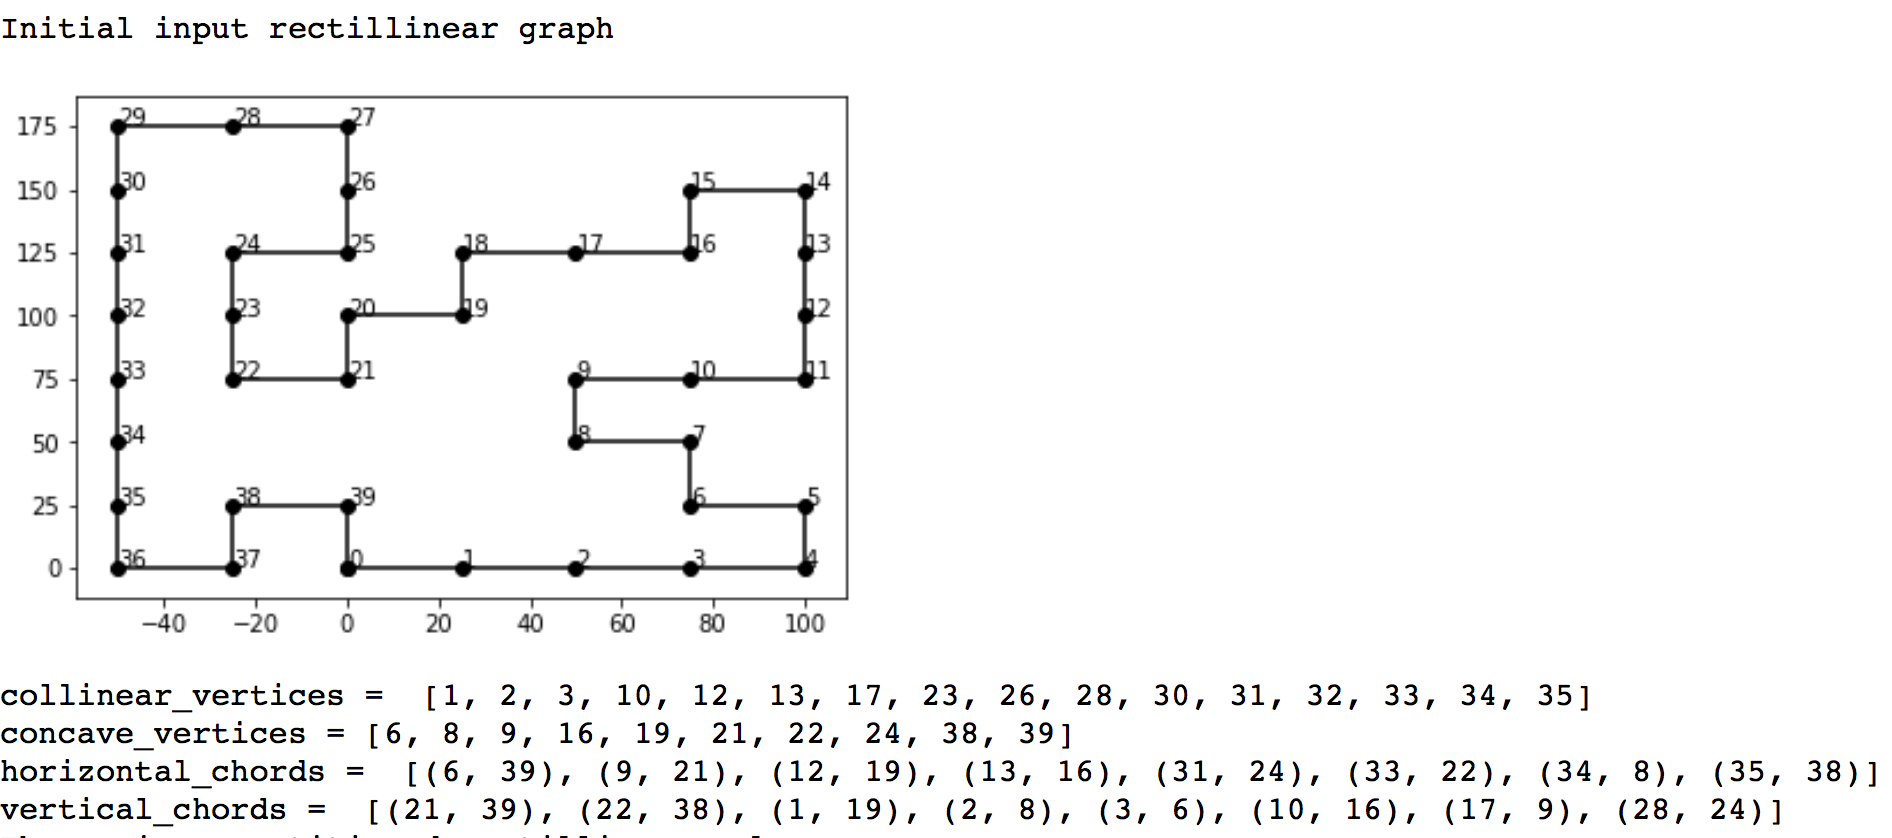
\includegraphics{Figures/t21.png}}
\end{figure}

\textbf{OUTPUT 2} 

\begin{figure}[h]
  \flushleft
  \scalebox{0.5}{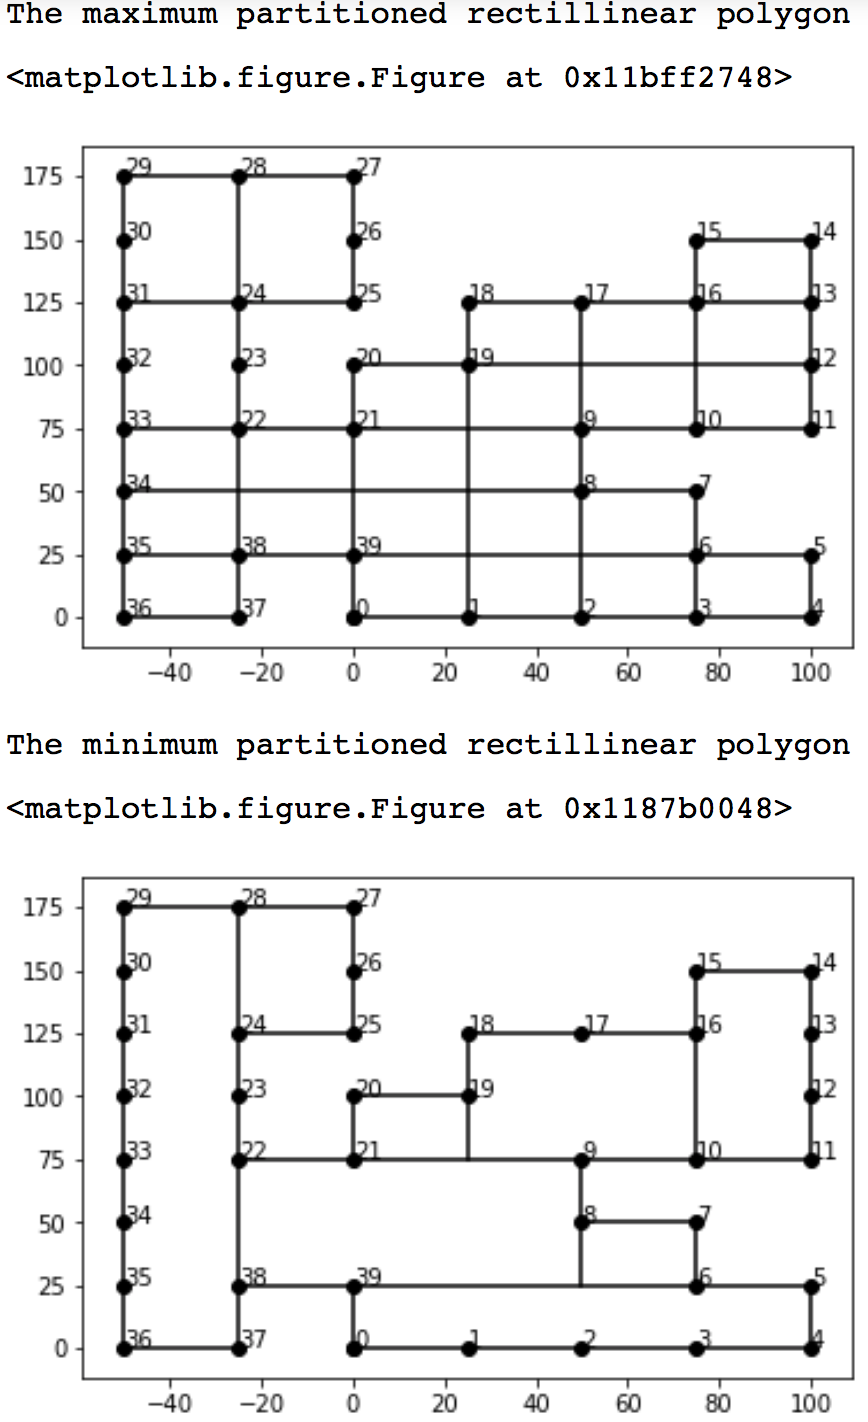
\includegraphics{Figures/t22.png}}
\end{figure}

\pagebreak
\textbf{INPUT 3}

\begin{figure}[h]
  \centering
  \scalebox{0.45}{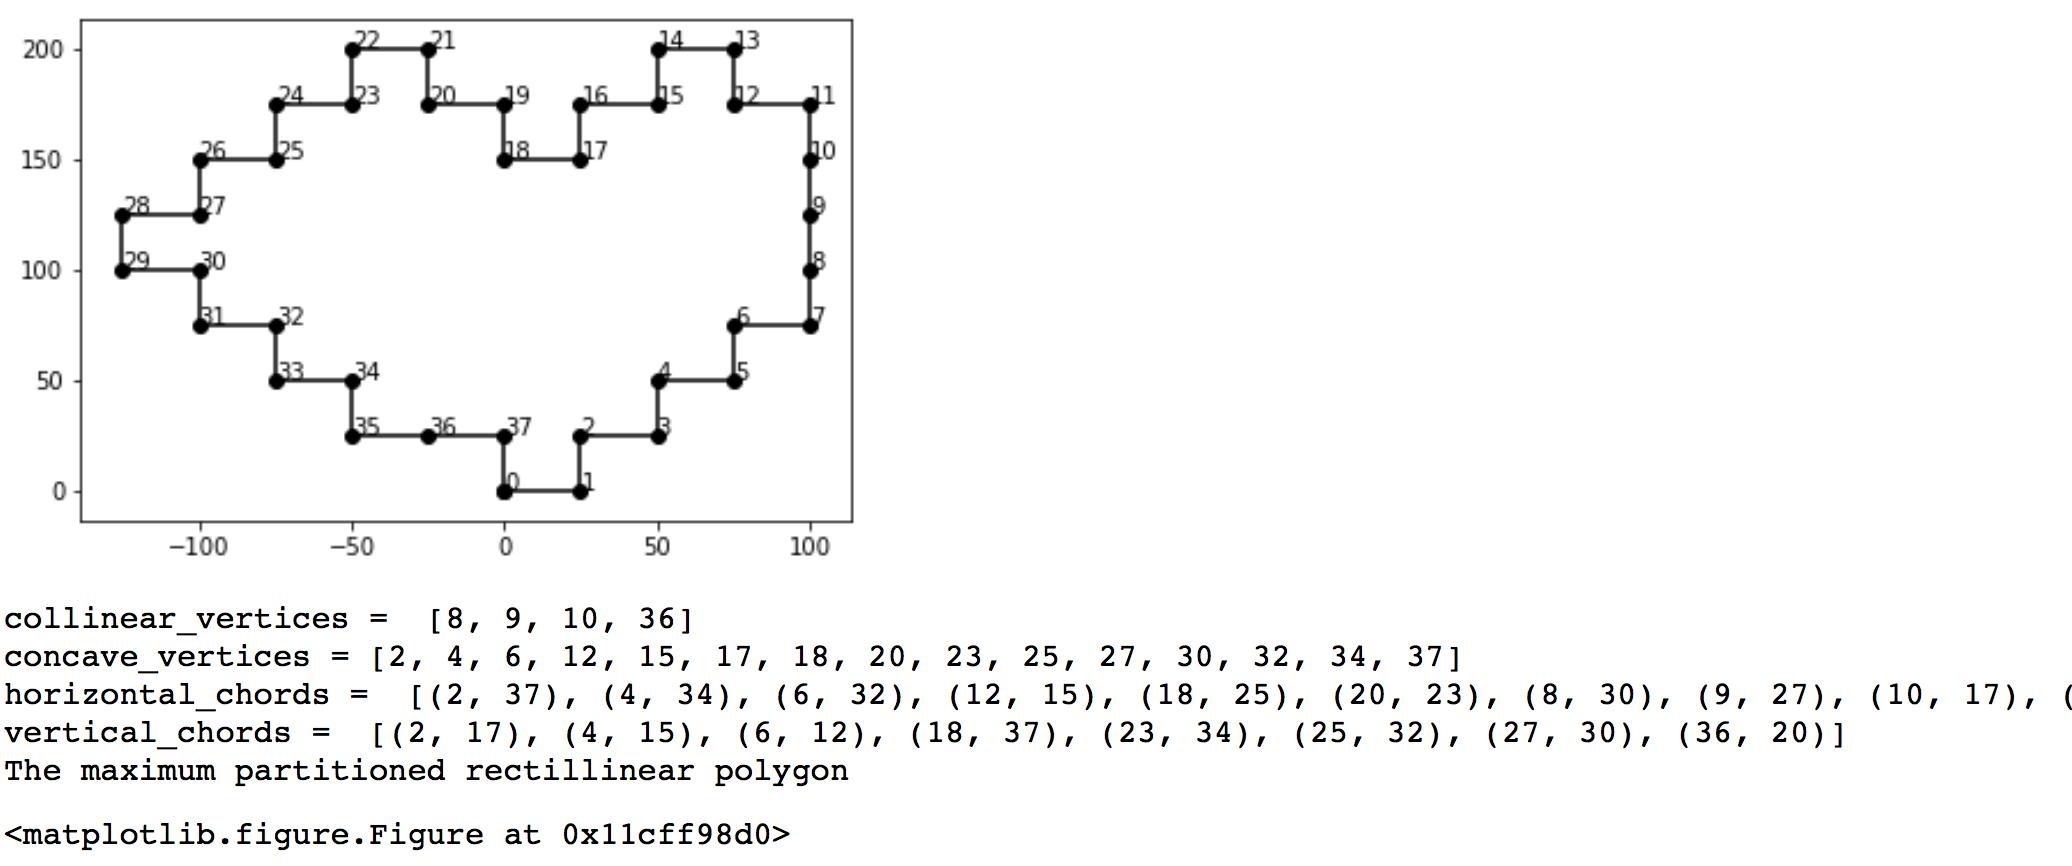
\includegraphics{Figures/t31.png}}
\end{figure}

\textbf{OUTPUT 3} 

\begin{figure}[h]
  \flushleft
  \scalebox{0.5}{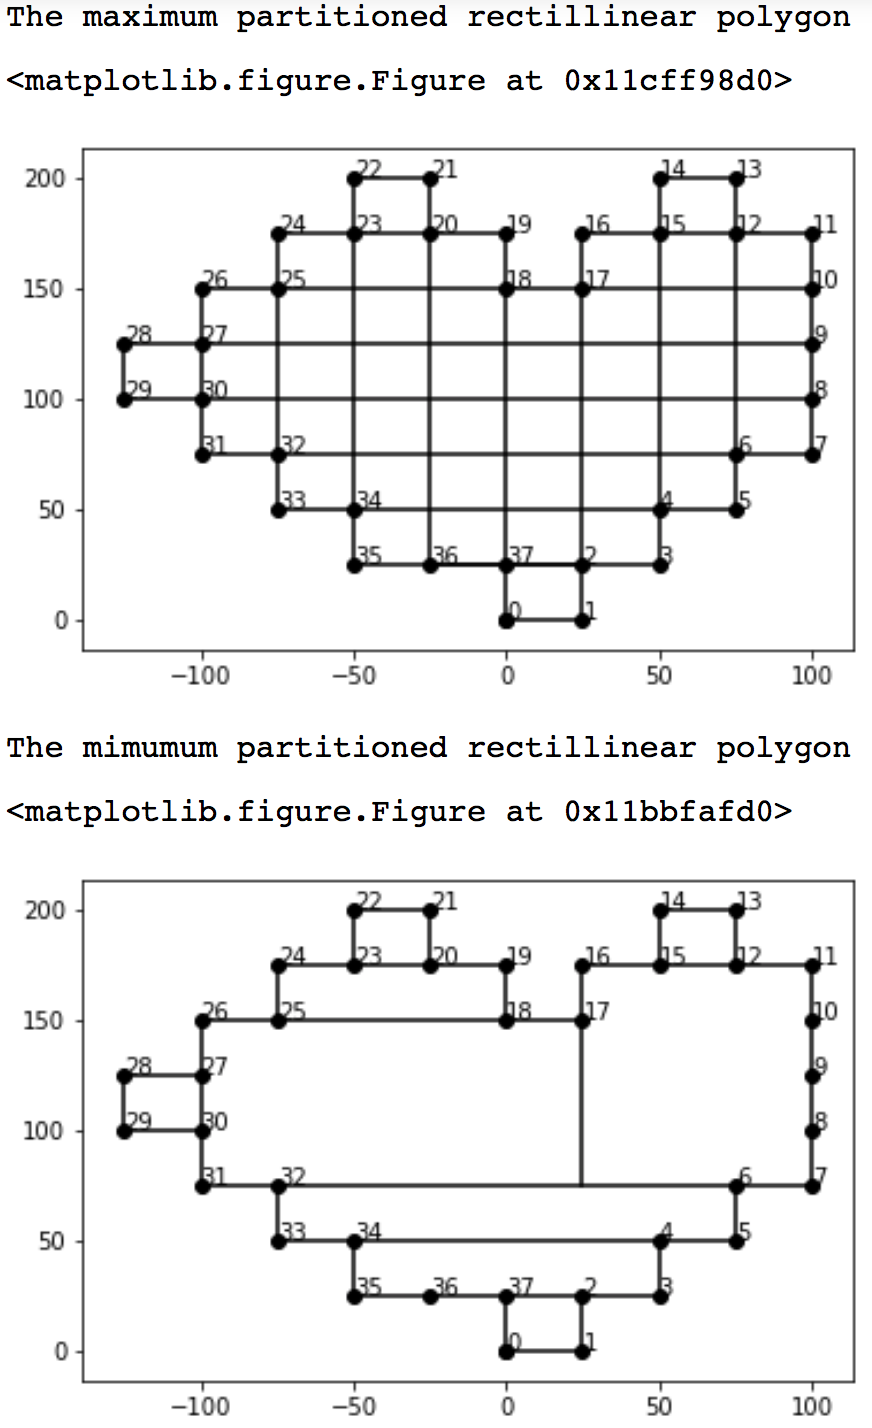
\includegraphics{Figures/t32.png}}
\end{figure}

\pagebreak
\textbf{INPUT 4}

\begin{figure}[h]
  \centering
  \scalebox{0.45}{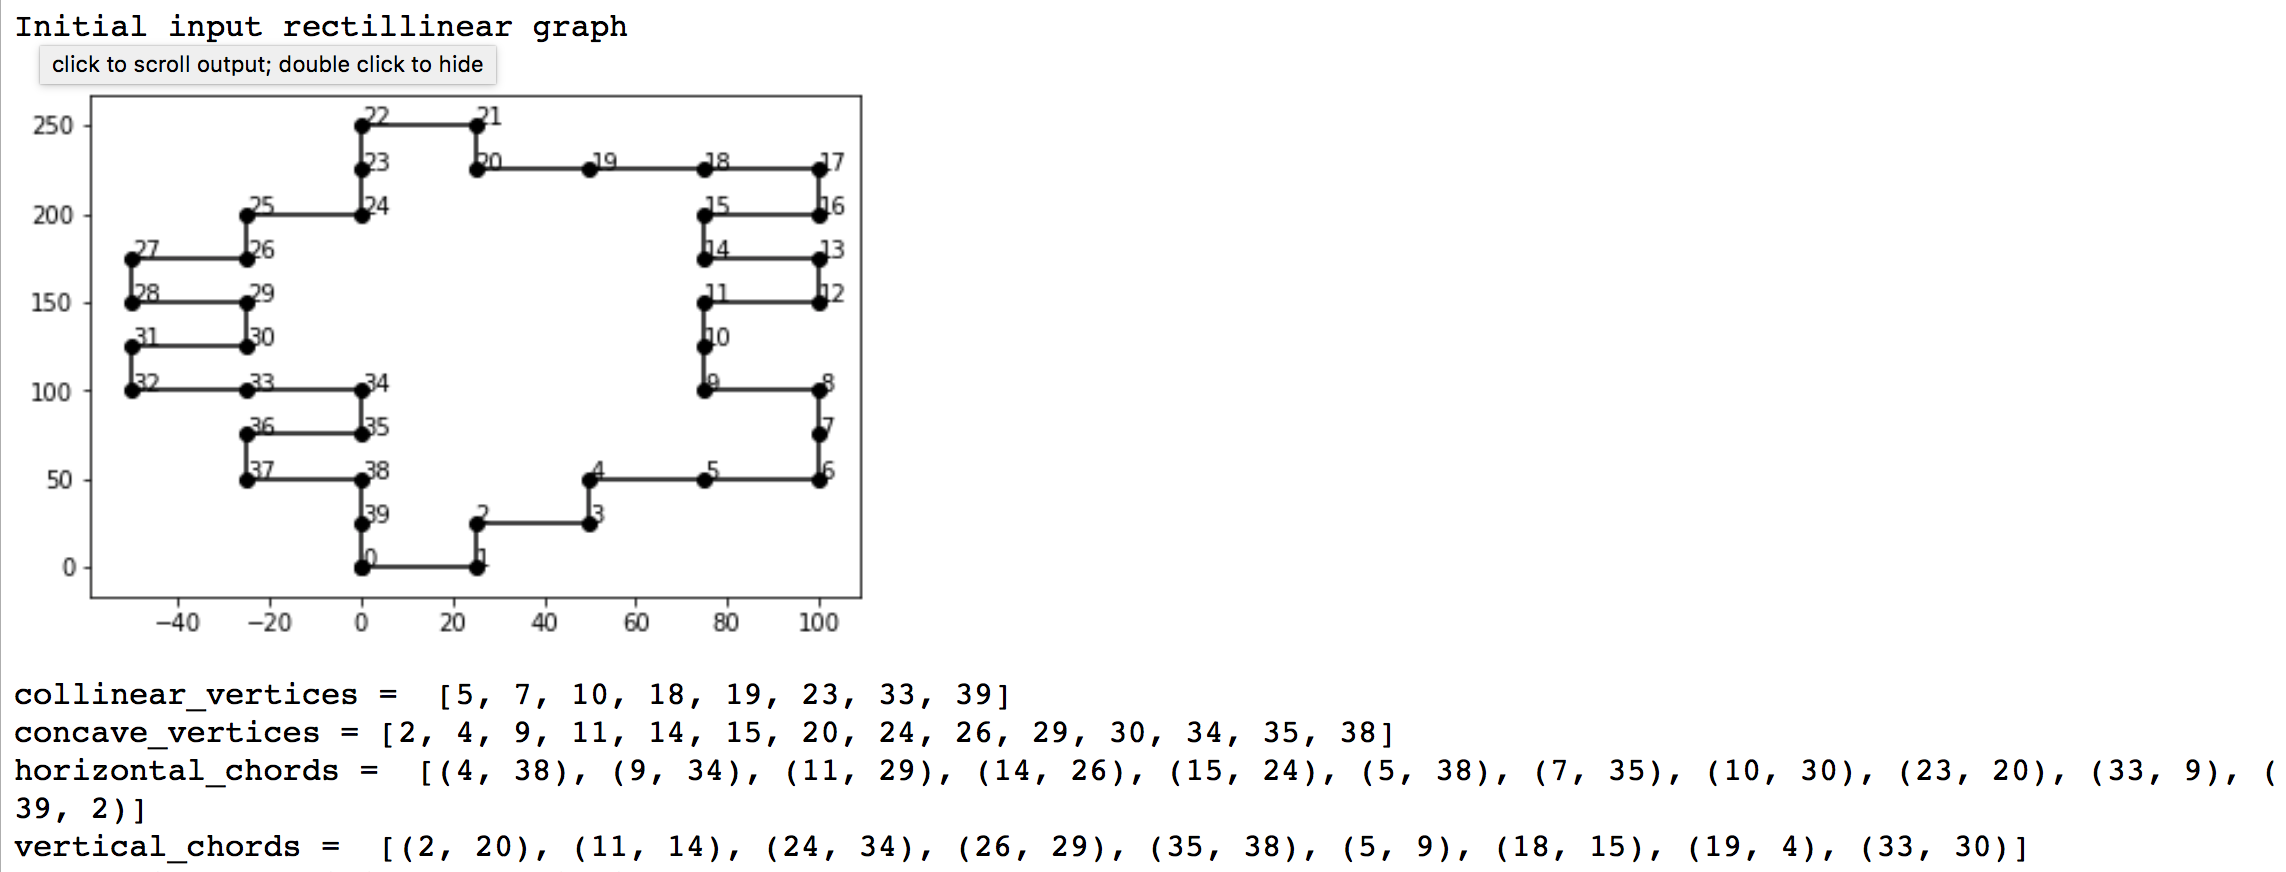
\includegraphics{Figures/t41.png}}
\end{figure}

\textbf{OUTPUT 4} 

\begin{figure}[h]
  \flushleft
  \scalebox{0.5}{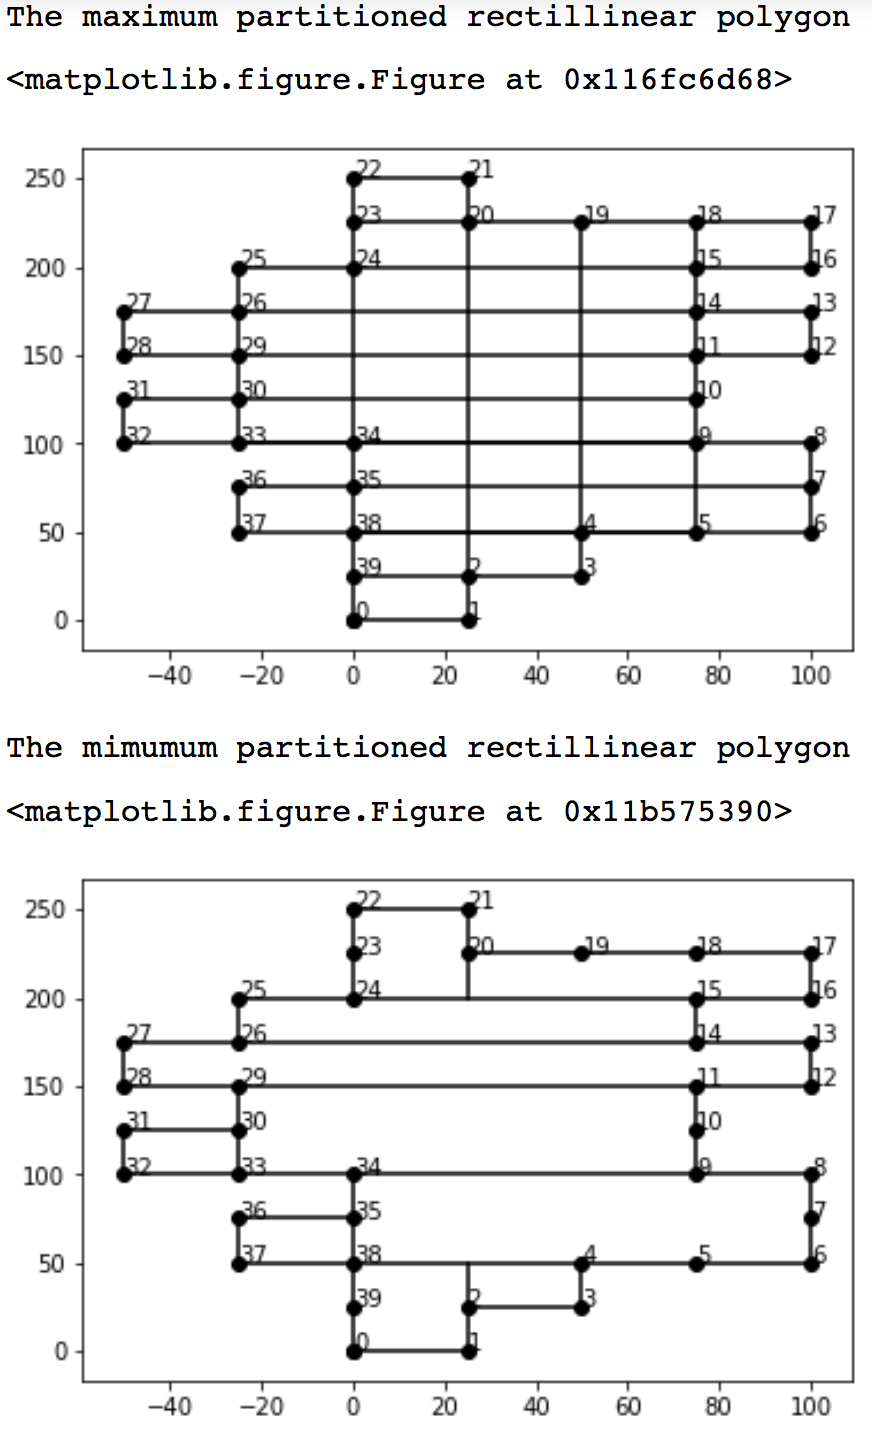
\includegraphics{Figures/t42.png}}
\end{figure}
%---------------------------------------------------

\chapter{Conclusion}
\label{Conclusion}
\lhead{Conclusion}

The algorithm reviewed does not give unique solutions, as the maximum independent set is not itself unique. Since, the horizontal and vertical sets of chords themselves make up two different set of maximum independent set of chords, if the number of horizontal chords and vertical chords are equal. Also there can be other maximum independent set of chords.

My future work will involve working on problems related to applications of graph theory, involving similar but more complicated and self-motivated problems.

Thus, this implementation and design with the newest tools will help architects, in preparing their own architectural arrangements, according to their choice.